\begin{frame}
\frametitle{About This Work...}

\emph{Extracting Indoor Spatial Objects from CAD Models: A Database Approach}.~\cite{xu2015extracting} \\
D.~Xu, P.~Jin, X.~Zhang, J.~Du, and L.~Yue.\\~\\

\begin{itemize}
  \item propose a database approach to extracting indoor spatial objects from CAD models.
  \item further integrate them into an indoor moving-object database.
\end{itemize}

\end{frame}

%------------------------------------------------

\begin{frame}
\frametitle{Motivation}

\begin{itemize}
  \item A fundamental issue in indoor moving-object management is the construction of indoor-space maps~\cite{turner2014floor}
    \begin{fitemize}
      \item outdoor spaces have Google Maps and city road-network maps
      \item for indoor spaces, there are no existing solutions for automatically generating indoor maps
      \item manually draw the floor plan of an indoor space is time-consuming and costly
    \end{fitemize}

  \item present a database approach to automatically extract indoor spatial objects and generate indoor maps from CAD models
  \begin{fitemize}
    \item CAD is commonly used in indoor-space design
    \item resulting in a great number of CAD files depicting structure of buildings
  \end{fitemize}
\end{itemize}

\end{frame}

%------------------------------------------------

\begin{frame}
\frametitle{Drawing Exchange Format File}

CAD models are typically represented by the \conceptbf{Drawing Exchange Format}(DXF)~\cite{autoc77:online}.\\~\\

A DXF files stores in a key-value style: all the k-v pairs are organized into seven sections, namely \emph{HEADER}, \emph{CLASSES}, \emph{TABLES}, \emph{BLOCKS}, \emph{ENTITIES}, \emph{OBJECTS}, \emph{THUMBNAILIMAGE}.\\~\\

\emph{ENTITIES} section contains all graphical objects in the drawing.

\end{frame}

%------------------------------------------------

\begin{frame}
\frametitle{Data in Drawing Exchange Format File}

original data in DXF files are low-level graphical elements including \emph{points}, \emph{lines}, \emph{arcs}, \emph{ploylines} and \emph{circles}.\\~\\

However, one indoor spatial object may involve many graphical elements. Due to the large number of graphical elements in a file, it is not trivial to find the right elements that describe an outdoor spatial object.

\begin{columns}

  \column{0.45\textwidth}
  \begin{figure}[tb]
    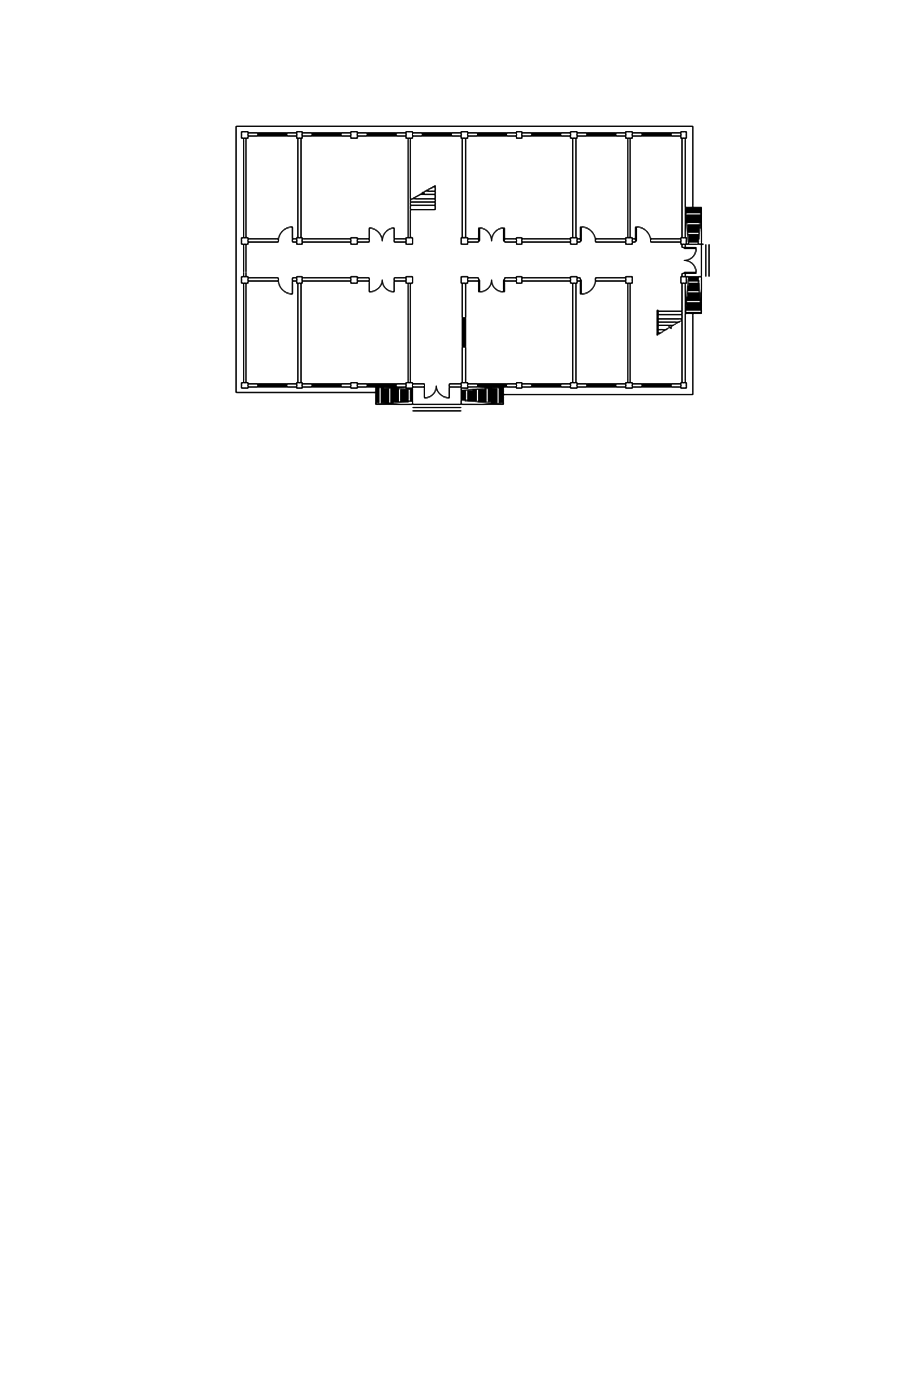
\includegraphics[width=0.9\columnwidth]{figures/2-8/2-8-1.pdf}
  \end{figure}

  \column{0.55\textwidth}
  \fsize{\textrm{in the example right, the walls of a room are separated by some arcs, lines and white squares, it is not feasible to simply extract rooms from CAD models}}

\end{columns}

\end{frame}

%------------------------------------------------

\begin{frame}
\frametitle{Problem State}

\begin{problem}[Extracting CAD Spatial Objects]
  Given a CAD model (DXF file), return a set of rooms, doors, and the topological relationship between doors and rooms, where each room is represented as a polygon, each door is represented as a point, and each topological relationship is a pair of (door, room) indicating that a door is connected with a room.
\end{problem}

\end{frame}

%------------------------------------------------

\begin{frame}
\frametitle{The Proposed Method: Basic Idea}

\textbf{DOORS}~~As doors are usually represented by arcs, just simply extract all arcs as door candidates and further make a refinement to remove those candidates that are not connected with rooms (after rooms have been recognized)\\~\\

\textbf{ROOMS}~~A rule-based approach is used, considering the following two problems: 1. a room's wall may involve too many lines in CAD models; 2. rooms are not always rectangles and they may be more than one door associated.\\~\\

\textbf{BASIC IDEA}~~to first employ a line-reduction preprocessing to simplify the line set that composed of a room; after that, use a line-extending technique to divide the entire indoor space into a set of geometric shapes; finally, use an MBR-based method to remove duplicated rooms.

\end{frame}

%------------------------------------------------

\begin{frame}
\frametitle{The Proposed Method: Definitions}

\begin{definition}[point-point adjacency]
  Two points are adjacent if their Euclidean distance is below a predefined threshold $\alpha$
  \begin{equation}
    p \overset{adj}{\leftrightarrow} q \Leftrightarrow dist(p,q) \leq \alpha
  \end{equation}
\end{definition}

\begin{definition}[point-line adjacency]
  A point $p$ is adjacent to a line $ln(s,e)$ if there is a \emph{point-point adjacency} relation between $ln$'s start point or end point and $p$
  \begin{equation}
    p \overset{adj}{\leftrightarrow} ln \Leftrightarrow (p \overset{adj}{\leftrightarrow} s \textbf ~or~ p \overset{adj}{\leftrightarrow} s)
  \end{equation}
\end{definition}

\end{frame}

%------------------------------------------------

\begin{frame}
\frametitle{The Proposed Method: Difinitions}

\begin{definition}[line-line adjacency]
  Let $ln_1(s_1, e_1)$ and $ln_2(s_2, e_2)$ be two lines. $ln_1$ and $ln_2$ are adjancent if there is a \emph{point-line adjacency} relation between an end point of one of the two lines and another line.
  \begin{equation}
    ln_1 \overset{adj}{\leftrightarrow} ln_2 \Leftrightarrow (s_1 \overset{adj}{\leftrightarrow} ln_2 ~or~e_1 \overset{adj}{\leftrightarrow} ln_2) ~or~ (s_2 \overset{adj}{\leftrightarrow} ln_1 ~or~e_2 \overset{adj}{\leftrightarrow} ln_1)
  \end{equation}
\end{definition}

\begin{definition}[parallel lines]
  Let $ln_1(s_1, e_1)$ and $ln_2(s_2, e_2)$ be two lines. $ln_1$ and $ln_2$ are parallel such that they satisfy the following condition.
  \begin{equation}
    ln_1 \overset{par}{\leftrightarrow} ln_2 \Leftrightarrow dot\_product(ln_1, ln_2) - dist(s_1, e_1) \cdot dist(s_2,e_2) < \beta
  \end{equation}
\end{definition}

\end{frame}

%------------------------------------------------

\begin{frame}
\frametitle{The Proposed Method: Difinitions}

Distance between two lines are computed as follows
\begin{figure}[tb]
  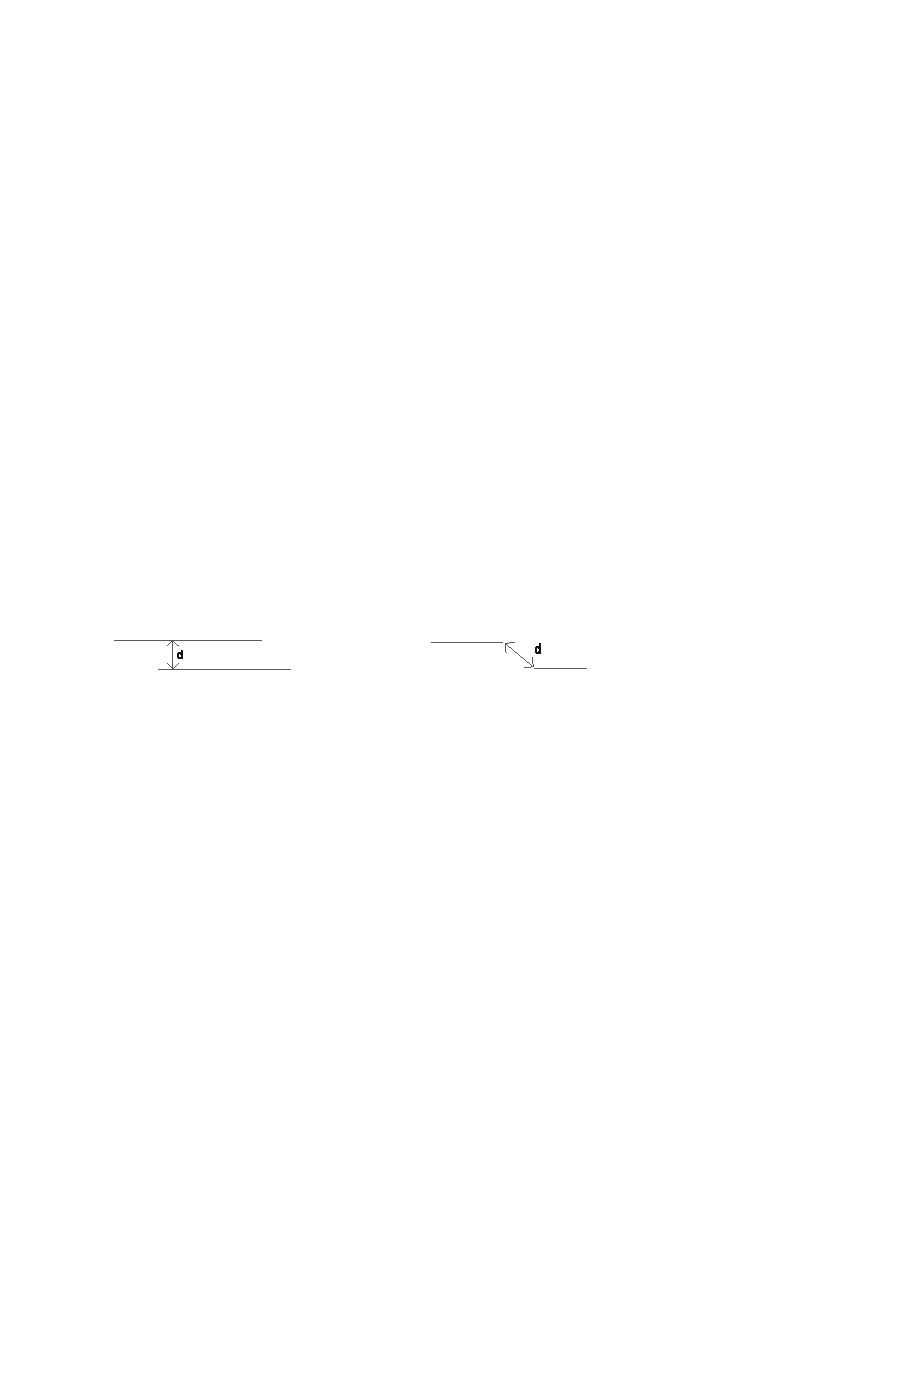
\includegraphics[width=\columnwidth]{figures/2-8/2-8-2.pdf}
\end{figure}

\begin{definition}[near lines]
  Two parallel lines are near if the distance between them is below a predefined threshold $\varepsilon$
\end{definition}

\end{frame}

%------------------------------------------------

\begin{frame}
\frametitle{The Proposed Method: Algorithm}

\begin{columns}

  \column{0.58\textwidth}
  \begin{figure}[tb]
    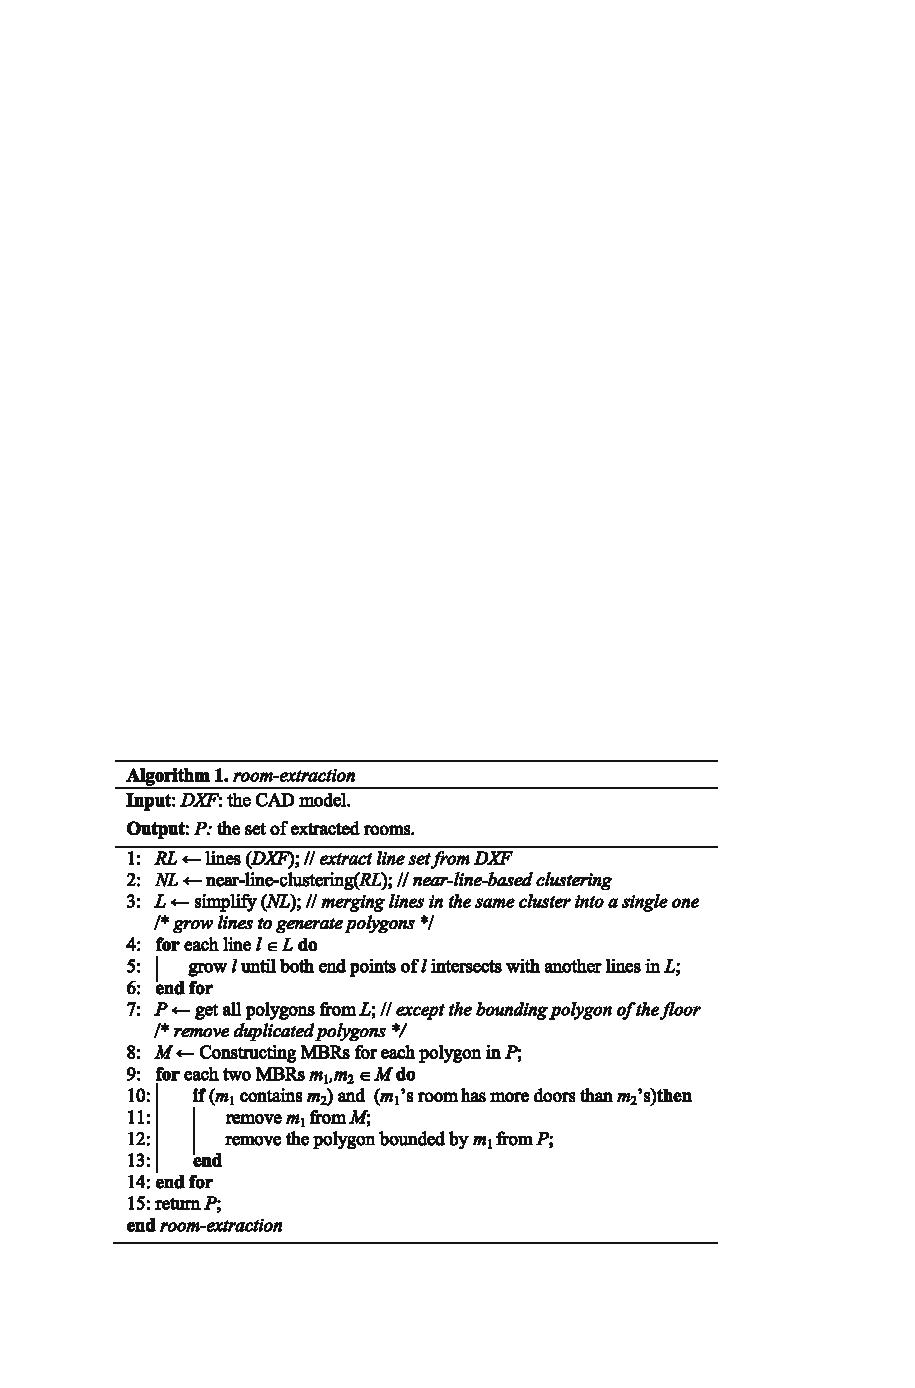
\includegraphics[width=\columnwidth]{figures/2-8/2-8-3.pdf}
  \end{figure}


  \column{0.42\textwidth}
  \ssize{
  \begin{enumerate}
    \item first obtain line clusters through a near-line-based clustering step
    \item simplify the lines in each cluster by merging near lines into a single line
    \item construct polygons using a line-growing technique, and then remove duplicated polygons by constructing MBRs for all polygons
    \item after extracting rooms, continue to refine door candidates that are extracted from arcs in the CAD model
    \item those candidates not connected with any rooms are removed from the door set.
  \end{enumerate}
  }

\end{columns}

\end{frame}

%------------------------------------------------

\begin{frame}
\frametitle{Integration into Indoor Moving-Object Databases}

Current relational database systems do not provide inherited support for complex object representation and storage. \\~\\

Object-relational database systems such as Oracle and PostgreSQL offer user-defined type extensions. \\~\\

Three indoor spatial types on Oracle, which are \emph{Indoor Position}, \emph{Indoor Space}, \emph{Indoor Geometry}. Oracle Spatial provides \emph{SDO\_GEOMETRY} for representing spatial data.

\end{frame}

%------------------------------------------------

\begin{frame}
\frametitle{Integration into Indoor Moving-Object Databases}

\textbf{Indoor Space} type describes rooms, doors, as well as the topological relationship between doors and rooms, representing as a tripe $(RoomSet, DoorSet, Room-Door)$. Where $RoomSet$ is the set of room identifiers, $DoorSet$ is the set of door identifiers, and $Room-Door$ represents the topological relationship between $RoomSet$ and $DoorSet$.\\~\\

\textbf{Indoor Geometry} type stores the exact geometric information about rooms and doors with the form $(ObjectID, Geo)$, where $ObjectID$ is a room ID or a door ID and $Geo$ is an \emph{SDO\_GEOMETRY} type supported by Oracle Spatial.

\end{frame}
